\documentclass[12pt]{article}
\usepackage{lecture}
\usepackage{html}
\usepackage{url}
\usepackage{graphics}
\usepackage{epstopdf}

\newcommand{\copyrightYears}{2001-2021}

\title{The Coalescent}

\begin{document}

\maketitle

\thispagestyle{first}

\section*{Introduction}

I've mentioned many times by now that population geneticists often
look at the world backwards. To those of you who aren't population
geneticists,\footnote{i.e., virtually everyone who is reading these
  notes.} looking at the world backwards is probably as awkwards as
walking backwards. Sometimes, though, it turns out that walking
backwards is useful, as when you're trying to keep an eye on where
you've been, not just where you're going. That's what we're about to
do with genetic drift. So far we've been trying to predict what will
happen in a population given a particular effective population
size. But when we collect data we are often more interested in
understanding the processes that produced the pattern we find than in
predicting what will happen in the future. We're using data to provide
insight about where we've been, not where we're going. So let's take a
backward look at drift and see what we find.


\section*{Reconstructing the genealogy of a sample of
  alleles}\index{allele genealogy}\index{coalescent}

Specifically, let's keep track of the genealogy of alleles. In a
finite population, two randomly chosen alleles will be identical by
descent with respect to the immediately preceding generation with
probability $1/2N_e$. That means that there's a chance that two
alleles in generation $t$ are copies of the same allele in generation
$t-1$. If the population size is constant, meaning that the number of
allele copies\footnote{I'm using the phrase ``allele copy'' here to
  refer to distinct physical alleles. Allele copies may or may not be
  identical by type or identical by descent. If a diploid population
  has effective size $N_e$, then the number of allele {\it copies\/}
  is $2N_e$. The number of allele types may be 1, 2, or any other
  integer less than or equal to $2N_e$. Similarly, the number of
  identity by descent categories among the alleles may be anything rom
  1 to $2N_e$.}\index{allele copy} is also constant, that also means
that there's a chance that some allele copies present in generation
$t-1$ will not have descendants in generation $t$. Looking backward,
then, the number of allele copies in generation $t-1$ that have
descendants in generation $t$ is always less than or equal to the
number of allele copies in generation $t$. That means if we trace the
ancestry of allele copies in a sample back far enough, all of them
will be descended from a single common ancestor.\footnote{As you can
  see, it quickly becomes tedious to write ``allele copies.'' I'm
  going to write ``allele'' throughout the rest of this
  discussion. Just remember that when I do, I'm really referring to an
  allele copy.}  Figure~\ref{fig:coalescent} provides a simple
schematic illustrating how this might happen.

\begin{figure}
\begin{center}
\resizebox{!}{5cm}{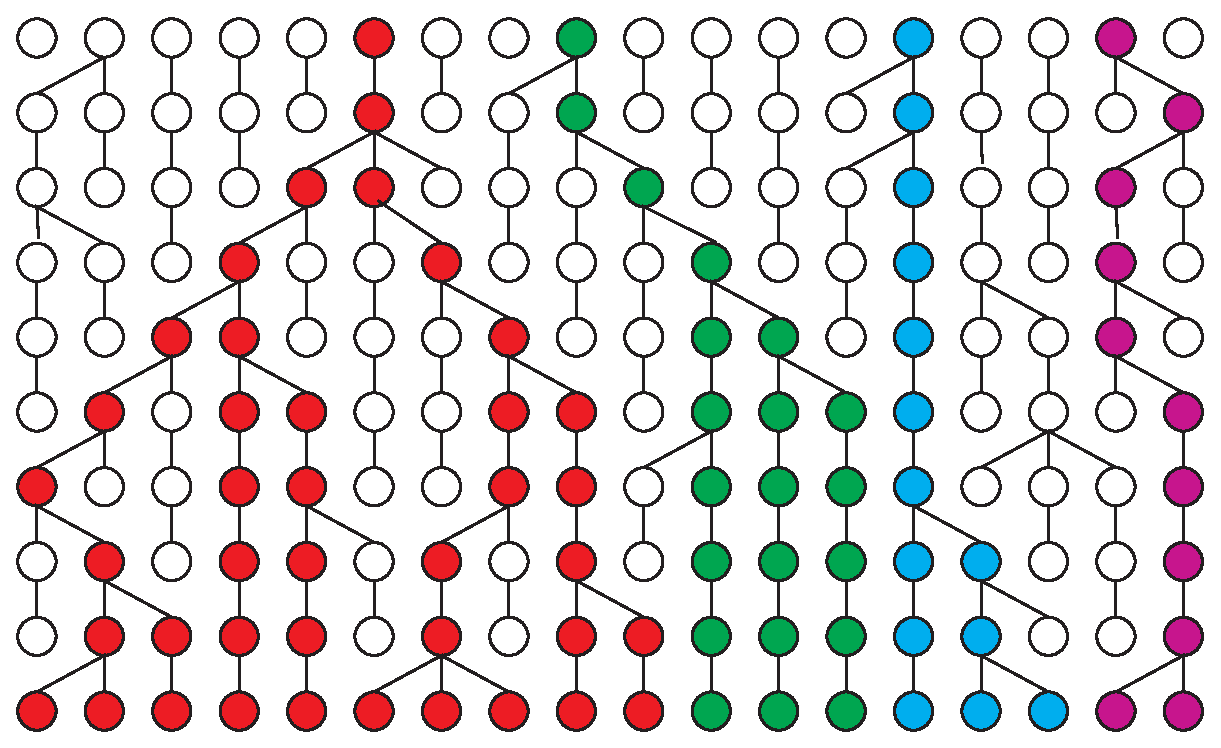
\includegraphics{coalescent-figure.eps}}
\end{center}
\caption{A schematic depiction of one possible realization of the
  coalescent process in a population with 18 haploid gametes. There
  are four coalescent events in the generation immediately preceding
  the last one illustrated, one involving three alleles.}\label{fig:coalescent}
\end{figure}

Time runs from the top of Figure~\ref{fig:coalescent} to the bottom,
i.e., the current generation is represented by the circles in the
botton row of the figure. Each circle represents an allele. The
eighteen alleles in our current sample are descended from only four
alleles that were present in the populations ten generations ago. The
other fourteen alleles present in the population ten generations ago
left no descendants. How far back in time we'd have to go before all
alleles are descended from a single common ancestor depends on the
effective size of the population, because how frequently two (or more)
alleles are descended from the same allele in the preceding generation
depends on the effective size of the population, too. But in any
finite population the pattern will look something like the one I've
illustrated here.

\section*{Mathematics of the coalescent: two
  alleles\footnote{Remember, I'm
  talking about allele copies here.}}\index{coalescent!two alleles}

The mathematician J. F. C. Kingman developed a convenient and powerful
way to describe how the time to common ancestry is related to
effective population
size~\cite{Kingman-1982-genealogy,Kingman-1982-coalescent}. The
process he describes is referred to as the {\it coalescent}, because
it is based on describing the probability of {\it coalescent
  events},\index{coalescent events} i.e., those points in the
genealogy of a sample of alleles where two alleles are descended from
the same allele in the immediately preceding generation.\footnote{An
  important assumption of the coalescent is that populations are large
  enough that we can ignore the possibility that there is more than
  one coalescent event in a single generation. That also means that we
  also only allow coalescence between a pair of alleles, not three or
  more. In both ways the mathematical model of the process differs
  from the diagram in Figure~\ref{fig:coalescent}.}  Let's consider a
simple case, one that we've already seen, e.g., two alleles
drawn at random from a single population.

The probability that two alleles drawn at random from a population are
copies of the same allele in the preceding generation is also the
probability that two alleles drawn at random from that population are
identical by descent with respect to the immediately preceding
generation. We know what that probability is,\footnote{Though you may
not remember it.} namely
\[
\frac{1}{2N_e^{(f)}} \quad .
\]
I'll just use $N_e$ from here on out, but keep in mind that the
appropriate population size for use with the coalescent is the
inbreeding effective size. Of course, this means that the probability
that two alleles drawn at random from a population are {\it not\/}
copies of the same allele in the preceding generation is
\[
1 - \frac{1}{2N_e} \quad .
\]
We'd like to calculate the probability that a coalescent event
happened at a particular time $t$, in order to figure out how far back
in the ancestry of these two alleles we have to go before they have a
common ancestor. How do we do that?

Well, in order for a coalescent event to occur at time $t$, the two
alleles must have {\it not\/} have coalesced in the generations
preceding that.\footnote{Remember that we're counting generations
  backward in time, so when I say that a coalescent event occurred at
  time $t$ I mean that it occurred $t$ generations ago.} The
probability that they did not coalesce in the first $t-1$ generations
is simply
\[
\left(1 - \frac{1}{2N_e}\right)^{t-1} \quad .
\]
Then after having remained distinct for $t-1$ generations, they have
to coalesce in generation $t$, which they do with probability
$1/2N_e$. So the probability that two alleles chosen at random
coalesced $t$ generations ago is
\begin{equation}
P(T=t) = \left(1 -
\frac{1}{2N_e}\right)^{t-1}\left(\frac{1}{2N_e}\right) \quad .
\label{eq:two-allele}
\end{equation}
It's not too hard to show, once we know the probability distribution
in equation (\ref{eq:two-allele}), that the average time to
coalescence for two randomly chosen alleles is $2N_e$.\footnote{If
  you've had a little bit of probability theory, you'll notice that
  equation~\ref{eq:two-allele} shows that the coalescence time is a
  geometric random variable.}\index{coalescent!time to common ancestry}

\section*{Mathematics of the coalescent: multiple
  alleles}\index{coalescent!multiple alleles}

It's quite easy to extend this approach to multiple
alleles.\footnote{Okay, okay. What I should really have said is ``It's
  not {\it too\/} hard to extend this approach to multiple alleles, if
  you are comfortable with probability thinking.'' Remember: I don't
  expect you to be able to derive these results on your own. Don't
  worry if you can't see how you could have come up with the
  mathematics that follow. Unless you want to make contributions to
  developing new theory in population genetics, you don't need to do
  derivations like these. Nonetheless, I think it's useful for you to
  see them. That way you have a better chance of understanding the
  limitations of coalescence approaches if you use them in analyzing
  your own data.}  We're interested in seeing how far back in time we
have to go before all alleles are descended from a single common
ancestor. We'll assume that we have $m$ alleles in our sample. The
first thing we have to calculate is the probability that any two of
the alleles in our sample are identical by descent from the
immediately preceding generation. To make the calculation easier, we
assume that the effective size of the population is large enough that
the probability of two coalescent events in a single generation is
vanishingly small. We already know that the probability of a
coalescence in the immediately preceding generation for two randomly
chosen alleles is $1/2N_e$. But there are $m(m-1)/2$ different pairs
of alleles in our sample.\footnote{Where did I get that $m(m-1)/2$?
  You can either take my word for it as ``a well known fact,'' or you
  can ask me about it, and I'll show you where it comes from.} So the
probability that one pair of these alleles is involved in a coalescent
event in the immediately preceding generation is
\begin{equation}
  \left(\frac{1}{2N_e}\right)\left(\frac{m(m-1)}{2}\right) \quad .
  \label{eq:multi-allele-first-event}
\end{equation}
From this it follows\footnote{Using logic just like what we used in
the two allele case.} that the probability that the first coalescent
event involving this sample of alleles occurred $t$ generations ago is
\begin{equation}
P(T=t) =
\left(1-\left(\frac{1}{2N_e}\right)\left(\frac{m(m-1)}{2}\right)\right)^{t-1}
\left(\frac{1}{2N_e}\right)\left(\frac{m(m-1)}{2}\right)
\quad .
\label{eq:multi-allele}
\end{equation}
So the mean time back to the first coalescent event is
\[
\frac{2N_e}{m(m-1)/2} = \frac{4N_e}{m(m-1)} \hbox{ generations} \quad .
\]

But this is, of course, only the first coalescent event. We were
interested in how long we have to wait until {\it all\/} alleles are
descended from a single common ancestor. Now this is where Kingman's
sneaky trick comes in. After the first coalescent event, we have $m-1$
alleles in our sample, instead of $m$. So the whole process starts
over again with $m-1$ alleles instead of $m$.\footnote{For anyone who
  cares, this is another example of the Markov property of genetic
  drift.}\index{genetic drift!Markov property} Since the time to the
first coalescence depends only on the number of alleles in the sample
and not on how long the first coalescence event took, we can calculate
the average time until all coalescences have happened
as\index{coalescent!time to coalescence}
\begin{eqnarray*}
\bar t &=& \sum_{k=2}^m \bar t_k \\
       &=& \sum_{k=2}^m \frac{4N_e}{k(k-1)} \\
       && \mbox{TAMO} \\
       &=& 4N_e\left(1 - \frac{1}{m}\right) \\
       &\approx& 4N_e
\end{eqnarray*}

\subsection*{A continuous time version of the coalescent}

Since the effective size of a population has to be pretty big for the
coalescent process to be a good representation, big enough that
$(1/2N_e)^2$ is negligible, $4N_e$ is generally in the hundreds or
thousands. That means that even though the coalescent as I formulated
it above is a discrete time process, i.e., events happen at time 1, 2,
3, $\dots$, it can be convenient to think of time as continuous, which
is surprisingly easy to do. We start with the ``well-known fact'' that
if $p$ is ``small''
\[
\log(1-p) \approx -p \quad .
\]
As a result,
\begin{eqnarray*}
(1 - p)^t &=& e^{t \log(1-p)} \\
          &\approx& e^{-pt} \quad .
\end{eqnarray*}
In our case,
\[
p = \frac{k(k-1)}{4N_e} \quad ,
\]
when there are $k$ alleles.\footnote{Remember, I'm using ``alleles''
  as shorthand for ``allele copies'' (and wasting a lot more space
  with this footnote than I would have if I'd just written ``allele
  copies'' in the text).} So
\[
t_k = \left(\frac{k(k-1)}{4N_e}\right)e^{{(t-1)}{\frac{k(k-1)}{4N_e}}} \quad .
\]


\subsection*{An example: Mitochondrial
  Eve}\index{coalescent!mitochondrial Eve}

Cann et al.~\cite{Cann-etal-1987} sampled mitochondrial DNA from 147
humans of diverse racial and geographic origins.\footnote{That may
  seem like a pretty small sample to you, but the technology
  available to analyze genomes has advanced tremendously since Cann et
  al. did their work. To sequence a segment of DNA for example,
  required, among other things, running samples on a polyacrylamide
  gel, producing an autoradiogram, and manually reading the
  results. The process took about 2 weeks per sequence.}  Based on the
amount of sequence divergence they found among genomes in their sample
and independent estimates of the rate of sequence evolution, they
inferred that the mitochondria in their sample had their most recent
common ancestor about 200,000 years ago. Because all of the most
ancient lineages in their sample were from individuals of African
ancestry, they also suggested that mitochondrial Eve lived in
Africa. They used these arguments as evidence for the ``Out of
Africa'' hypothesis for modern human origins, i.e., the hypothesis
that anatomically modern humans arose in Africa about 200,000 years
ago and displaced other members of the genus {\it Homo\/} in Europe
and Asia as they spread. What does the coalescent tell us about their
conclusion?

Well, we expect all mitochondrial genomes in the sample to have had a
common ancestor about $2N_e$ generations ago. Why $2N_e$ rather than
$4N_e$? Because mitochondrial genomes are haploid, not
diploid. Furthermore, since we all get our mitochondria from our
mothers,\footnote{Luo et al.~\cite{Luo-etal-2018} recently presented
  data suggesting that mitochondria may sometimes be biparentally
  inherited in humans and that whether or not biparental inheritance
  occurs seems to be determined by the nuclear genotype of the
  mother.} $N_e$ in this case refers to the effective number of {\it
  females}.

Given that a human generation is about 20 years, a coalescence time of
200,000 years implies that the mitochondrial genomes in the Cann et
al. sample have their most recent common ancestor about 10,000
generations ago. If the effective number of females in the human
populations is 5000, that's exactly what we'd expect. While 5000 may
sound awfully small, given that there are more than 3 billion women on
the planet now, remember that until the recent historical past (no
more than 500 generations ago) the human population was small and
humans lived in small hunter-gatherer groups, so an effective number
of females of 5000 and a total effective size of 10,000 may not be
unreasonable. If that's true, then the geographical location of
mitochondrial Eve need not tell us anything about the origin of modern
human populations, because there had to be a coalescence
somewhere. There's no guarantee, from this evidence alone, that the
Y-chromosome Adam would have lived in Africa, too. Having said that,
my limited reading of the literature suggests that more extensive
recent data are consistent with the ``Out of Africa''
scenario. Y-chromosome polymorphisms, for example, are also consistent
with the ``Out of Africa''
hypothesis~\cite{Underhill-etal-2000}. Interestingly, dating of
Y-chromosome polymorphisms suggests that Y-chromosome Adam left
Africa only 35,000 -- 89,000 years ago.

\section*{The coalescent and $F$-statistics}\index{F-statistics@$F$-statistics!coalescent}\index{coalescent!F-statistics@$F$-statistics}

Suppose we have a sample of alleles from a structured population. For
alleles chosen randomly within populations, let the average time to
coalescence be $\bar t_0$. For alleles chosen randomly from different
populations, let the average time to coalescence be $\bar t_1$. If
there are $k$ populations in our sample, the average time to
coalescence for two alleles drawn at random without respect to
population is\footnote{If you don't see why, don't worry about it. You
can ask if you really care. We only care about $\bar t$ for what
follows anyway.}
\begin{eqnarray*}
  \bar t &=& \frac{1}{k}\bar t_0 + \frac{k-1}{k}\bar t_1 \\
  &=& \frac{\bar t_0 + (k-1)\bar t_1}
              {k} \quad .
\end{eqnarray*}
Slatkin~\cite{Slatkin-1991} pointed out that $F_{st}$ bears a simple
relationship to average coalescence times within and among
populations. Given these definitions of $\bar t$ and $\bar t_0$,
\begin{eqnarray*}
  F_{st} &=& \frac{\bar t - \bar t_0}{\bar t} \quad .
\end{eqnarray*}
So another way to think about $F_{st}$ is as a measure of the
proportional increase in coalescence time that is due to populations
being separate from one another. One way to think about that
relationship is this: the longer it has been, on average, since
alleles in different populations diverged from a common ancestor, the
greater the chance that they have become different. An implication of
this relationship is that $F$-statistics, by themselves, can tell us
something about how recently populations have been connected, relative
to the within-population coalescence time, but they can't distinguish
between recent common ancestry that is due to migration among
populations and recent common ancestry that is due to a split between
populations.

A given pattern of among-population relationships might reflect a
migration-drift equilibrium, a sequence of population splits followed
by genetic isolation, or any combination of the two. If we are willing
to assume that populations in our sample have been exchanging genes
long enough to reach stationarity in the drift-migration process, then
$F_{st}$ may tell us something about migration. If we are willing to
assume that there's been no gene exchange among our populations, we
can infer something about how recently they've diverged from one
another. But unless we're willing to make one of those assumptions, we
can't really say anything.\index{genetic drift!migration}\footnote{We can't say anything from allele
  frequencies alone. If we have DNA sequences for the alleles, which
  allow us to tell how closely related they are to one another, we
  can say something. We'll get to this when we discuss phylogeography
  in a few weeks.}

\section*{The coalescent and natural selection}\index{coalescent!natural selection}

It shouldn't surprise you that if we can study some of the properties
of drift and selection, we can also use the coalescent to understand
how natural selection works in a finite population. Even though the
mathematics of the coalescent are ususally simpler than the older
diffusion approach for studying allele frequency changes in a finite
population, they are still very complicated. I'll simply outline one
approach here known as the {\it structured
  coalescent}.\index{structured coalescent} 

The idea is reasonably simple, especially if we think about selection
involving only two alleles.\footnote{Wakeley~\cite{Wakeley-2010}
  provides a reasonably accessible overview. Coop and
  Griffiths~\cite{Coop-Griffiths-2004} provide all of the gory
  details.} When you start to think about it, you should realize two
things pretty quickly:

\begin{enumerate}

  \item Coalescent events will happen only {\it within} each of the
    two allele classes. If we were to trace the history back far
    enough, to the point where the mutation leading to a second allele
    occurred, then there might be coalescence involving the two
    classes{\dash}except that there wouldn't be two classes, only
    one.

  \item The allele copies\footnote{There's that phrase again.} within
    one of the two allele classes will all have the same fitness
    properties. That means that the genealogy within each allele
    classs will behave just like the coalescent you've already seen.
    
 \end{enumerate}
There are a couple of further complications. The first one is that the
probability of a coalescent event between two alleles belonging to an
allele class whose frequency is $p_t$ is
\[
 \frac{\frac{m(m-1)}{2}}{2N_ep_t} \quad .
 \]
If you think about it a bit, that may look reasonably familiar. If it
doesn't, look back at equation~(\ref{eq:multi-allele-first-event}). All
we've done is to reduce the effective size of the population by a
factor $p_t$, which is the fraction of total allele copies that belong
to the allele class we're focusing on.

The second complication is hidden in the first one. Notice that
subscript on $p_t$. Since we're assuming that natural selection is
going on, we expect the allele frequencies to change over time. This
is where the mathematics get really complicated. Since the population
is finite, we can't simply calculate the trajectory. We have to
simulate it. That's OK because when applying coalescent ideas to make
inferences from data, we're always simulating anyway. It's just that
simulating a sample when there is selection is a bit more complicated.

\begin{enumerate}

  \item We first simulate the allele frequency trajectory, typically
    using our estimate of the current allele frequency as a starting
    point.

  \item Then we simulate the coalescent history within each allele
    class.

  \item The result is a {\it structured coalescent}\index{structured coalescent}  
    sample that we can use for further analyses. We'll talk more about
    how to use these simulated samples when we get to phylogeography.
    
  \end{enumerate}

\bibliography{popgen}
\bibliographystyle{plain}

\ccLicense

\end{document}
